\documentclass[8pt]{extarticle}
\usepackage{geometry}
% \usepackage{showframe}

\geometry{
    a4paper, 
    margin=0.3in
}

\usepackage{graphicx} % Required for inserting images
\usepackage{amsmath}
\usepackage{amsfonts}
\usepackage{preamble}
\usepackage{multicol}
\usepackage{lipsum}
\usepackage[framemethod=TikZ]{mdframed}
\usepackage{thmboxes}
\usepackage{float}
% \usepackage{setspace}
\usepackage[nodisplayskipstretch]{setspace}

% \setlength{\parskip}{0pt}

\begin{document}

\setlength{\abovedisplayskip}{5pt}
\setlength{\belowdisplayskip}{5pt}
\setlength{\abovedisplayshortskip}{5pt}
\setlength{\belowdisplayshortskip}{5pt}

\section{\huge Algebra}
\begin{multicols}{2}
\raggedcolumns
\subsection*{Functions and Symmetries}

\begin{dfn}[Functions]{def:functions}{0.1.1}
A function $f:X\to Y$ is called
\renewcommand\labelitemi{\tiny$\bullet$}
\begin{itemize}
    \setlength\itemsep{0em}
    \item \textbf{injective} if $f(x_{1}) = f(x_{2}) \implies x_{1} = x_{{2}}$
    \item \textbf{surjective} if for every $y\in Y,\, \exists x\in X$ s.t. $f(x) = y$
    \item \textbf{bijective} if it is both injective and surjective
\end{itemize}
% \begin{figure}[H]
%     \centering
%     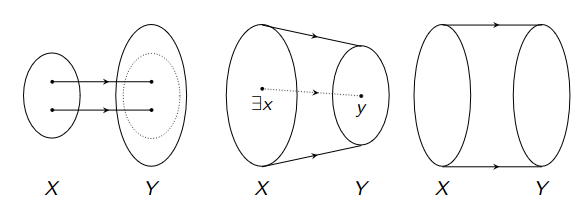
\includegraphics[width=\linewidth]{images/functions.png}
% \end{figure}
\end{dfn}
\vspace{-5pt}

\begin{dfn}[Graph Isomorphisms]{def:graph-iso}{1.1.3}
    An \textbf{isomorphism} between two graphs is a \textit{bijection} between them that preserves all edges. More precisely, if $\Gamma_{1}$ and $\Gamma_{2}$ are graphs, with sets of vertices $V_{1}$ and $V_{2}$ respectively, then an isomorphism from $\Gamma_{1}$ and $\Gamma_{2}$ is a bijection
    \[f : V_{1}\to V_{2}\]
    such that $f(v_{1})$ and $f(v_{2})$ are joined by an edge if and only if $v_{1}$ and $v_{2}$ are also joined by an edge.
    We say that $\Gamma_{1}$ and $\Gamma_{2}$ are \textit{isomorphic} if there exists an isomorphism $f:\Gamma_{1}\to\Gamma_{2}$
\end{dfn}
\vspace{-5pt}

\begin{dfn}[Symmetry]{def:symmetry}{1.1.9}
    A \textbf{symmetry} of a graph is an \textit{isomorphism} from the graph to itself, i.e. if the set of vertices is V, then the symmetry is a bijection $f:V\to V$ that preserves edges. That is, a symmetry is a bijection $f:V\to V$ such that $f(v_{1})$ and $f(v_{2})$ are joined by an edge if and only if $v_{1}$ and $v_{2}$ are joined by an edge.
\end{dfn}
\vspace{-5pt}

% -------------------------------------

\subsection*{Groups}

\begin{dfn}[Groups]{def:group-def}{1.2.3}
    For an operation $\ast$, We say a non-empty set G is a \textbf{group} under $\ast$ if the following four axioms hold:
    \renewcommand\labelitemi{\tiny$\bullet$}
    \begin{itemize}
        \setlength\itemsep{0em}
        \item \textbf{G1 - Closure:} $\ast$ is a binary operation on G, that is $a\ast b \in G$ for all $a,b\in G$.
        \item \textbf{G2 - Associativity:} $(a\ast b) \ast c =a\ast(b\ast c)$ for all $a,b,c\in G$
        \item \textbf{G3 - Identity:} There exists an \textit{identity} element of $G$ such that $e\ast g = g\ast e = e$ for all $g\in G$.
        \item \textbf{G4 - Inverse:} Every element $g\in G$ has an *inverse* $g^{-1}$ such that $g\ast g^{-1}=g^{-1}\ast g = e$
    \end{itemize}
\end{dfn}
\vspace{-5pt}

\begin{dfn}[Abelian Group]{def:abelian}{1.2.6}
    The definition of a group doesn't require that $a\ast b = b\ast a$.
    We say that a group is \textbf{abelian} or \textbf{commutative} if $a\ast b = b\ast a$ for every $a,b\in G$. We say that $a$ \textit{commutes} with $b$, or that $a$ and $b$ \textit{commute}
\end{dfn}
\vspace{-5pt}

% TODO: Examples of groups
% Dihedral, Symmetric, Product Group, Sets of numbers

% -------------------------------------

\subsection*{Subgroups}

\begin{dfn}[Subgroups]{def:subgroup-def}{2.1.1}
    Let $G$ be a group. We say that a non-empty subset $H$ of $G$ is a \textbf{subgroup} of $G$ if $H$ itself is a group (under the operation from $G$). We write $H\le G$ if $H$ is a subgroup of $G$. If $H\ne G$, we write $H<G$ and say $H$ is a proper subgroup
\end{dfn}
\vspace{-5pt}

\begin{thm}[Subgroup Test]{thm:subgroup-test}{2.1.3}
    $H\subseteq G$ is a subgroup of $G$ if and only if:
    \renewcommand\labelitemi{\tiny$\bullet$}
    \begin{itemize}
        \setlength\itemsep{0em}
        \item \textbf{S1:} $H$ is not empty
        \item \textbf{S2:} If $h,k\in H$ then $h\ast k\in H$
        \item \textbf{S3:} If $h\in H$ then $h^{-1}\in H$
    \end{itemize}
    Alternative test for subgroups:
    \renewcommand\labelitemi{\tiny$\bullet$}
    \begin{itemize}
        \setlength\itemsep{0em}
        \item $\widetilde{S1}$: $H$ is not empty.
        \item $\widetilde{S2}$: If $h,k\in H$ then $h*k^{-1}\in H$
    \end{itemize}
\end{thm}
\vspace{-5pt}

\begin{dfn}[Order of an Element]{def:element-order}{2.2.4}
    Let $G$ be a group and $g\in G$. Then the \textbf{order} $o(g)$ of $g$ is the \textit{least} natural number $n$ such that
    $$g^n = e$$
    If no such $n$ exists, we say that $g$ has infinite order
\end{dfn}
\vspace{-5pt}

\begin{dfn}[Order of a Group]{def:group-order}{2.2.3}
    The \textbf{order} of a finite group, written $\lvert G \rvert$, is the number of elements in $G$.
    If $G$ is infinite we say that $\lvert G \rvert = \infty$, or the order of $G$ is infinite.
\end{dfn}
\vspace{-5pt}

\begin{thm}[Order of a Finite Group]{thm:finite-order-thm}{2.2.6}
    In a finite group, every element has finite order.\newline
    If $g$ is an element of a finite group $G$, then there exists $k\in \N$ such that $g^{k} = g^{-1}$
\end{thm}
\vspace{-5pt}

\begin{dfn}[Generating Subset]{def:generator}{2.2.8}
    Let $G$ be a group and let $g\in G$ be an element. We define the subset
    $$\langle g \rangle := \{g^k \mid k\in\mathbb{Z}\} = \{\dots,\,g^{-2},\,g^{-1},\,e,\,g,\,g^{2},\,\dots \}$$
    Note that if $G$ is finite, then by \ref{thm:finite-order-thm} $\langle g \rangle$ is finite, and we can think of $\langle g \rangle$ as
    $$\langle g \rangle = \{e,\,g,\,\dots,\,g^{o(g)-1}\}$$
\end{dfn}
\vspace{-5pt}

\begin{dfn}[Cyclic Subgroup]{def:cyclic-subgroup}{2.2.10}
    A subgroup $H\le G$ is \textbf{cyclic} if $H = \langle h \rangle$ for some $h\in H$. In this case, we say that $H$ is the \textit{cyclic subgroup generated by h}. If $G=\langle g \rangle$ for some $g\in G$, then we say that the group $G$ is \textit{cyclic}, and that $g$ is a \textit{generator}.
\end{dfn}
\vspace{-5pt}

\begin{rem}[Consequences of Cyclic groups]{rem:cyclic-consequences}{2.2.12 - 16}
    \renewcommand\labelitemi{\tiny$\bullet$}
    \begin{itemize}
        \setlength\itemsep{0em}
        \item \textbf{2.2.12} If $g\in G$, then $o(g)=\lvert \langle g \rangle \rvert$
        \item \textbf{2.2.13:} If $G$ is cyclic, then $G$ is abelian.
        \item \textbf{2.2.14:} Let $G$ be a finite group. Then
        \[G \text{ is cyclic } \iff G \text{ has an element of order} \lvert  G\rvert \]
        \item \textbf{2.2.15:} Let $G$ be a cyclic group and let $H$ be a subgroup of $G$. Then $H$ is cyclic.
        \item \textbf{2.2.16:} Let $m,n\in \N$, let $G=\langle g \rangle$ be a cyclic group of order $m$ and $H=\langle h \rangle$ be a cyclic group of order $n$. Then
        $$G \times H \text{ cyclic} \iff m \text{ and } n \text{ are coprime (gcd(m,n) = 1)}$$
    \end{itemize}
\end{rem}
\vspace{-5pt}

% -------------------------------------

\subsection*{Cosets and Lagrange}

\begin{dfn}[Relation]{def:relation}{2.3.2}
    Let $X$ be a set, and $R$ a subset of $X\times X$; thus $R$ consists of some ordered pairs $(s,t)$ with $s,t\in X$. If $(s,t) \in R$ we write $s \sim t$ and say "$s$ is related to $t$". We call $\sim$ a \textbf{relation} on $X$.
\end{dfn}
\vspace{-5pt}

\begin{dfn}[Equivalence Relation]{def:equiv-relation}{2.3.2}
    \renewcommand\labelitemi{\tiny$\bullet$}
    \begin{itemize}
        \setlength\itemsep{0em}
        \item \textbf{Reflexive:} $x\sim x$ for all $x\in X$
        \item \textbf{Symmetric:} $x\sim y$ implies that $y\sim x$ for all $x,y\in X$
        \item \textbf{Transitive:} $x\sim y$ and $y\sim z$ implies that $x\sim z$ for all $x,y,z\in X$
    \end{itemize}
    A relation $\sim$ is called an \textbf{equivalence relation} on X if it satisfies the following three axioms:  
\end{dfn}
\vspace{-5pt}

\begin{dfn}[Coset]{def:coset}{2.3.4}
    Let $H\le G$ and let $g\in G$. Then a \textit{left coset} of  $H$ in $G$ is a subset of $G$ of the form $gH$, for some $g\in G$.
    We denote the set of left cosets of $H$ in $G$ by $G/H$
\end{dfn}
\vspace{-5pt}

\newpage

% -------------------------------------
% ==================================\equiv
% -------------------------------------

\begin{thm}[Coset Rules]{thm:coset-rules}{2.3.8}
Let $H\le G$
\renewcommand\labelitemi{\tiny$\bullet$}
\begin{itemize}
    \setlength\itemsep{0em}
    \item For all $h\in H$, $hH = H$. In particular $eH = H$
    \item For $g_{1}, g_{2}\in G$, the following are equivalent
    \renewcommand\labelitemi{\tiny$\bullet$}
    \begin{itemize}
        \setlength\itemsep{0em}
        \item $g_{1}H = g_{2}H$
        \item there exists $h\in H$ such that $g_{2} = g_{1}H$
        \item $g_{2}\in g_{1}H$
    \end{itemize}
    \item For $g_{1},\,g_{2}\in G$, define $g_{1}\sim g_{2}$ if and only if $g_{1}H=g_{2}H$. Then $\sim$ defines an equivalence relation on $G$.
\end{itemize}
\end{thm}
\vspace{-5pt}

\begin{thm}[Lagrange's Theorem]{thm:lagrange}{2.4.2}
Suppose that $G$ is a finite group.
\renewcommand\labelitemi{\tiny$\bullet$}
\begin{itemize}
    \setlength\itemsep{0em}
    \item If $H\le G$, then $\lvert  H\rvert $ divides $\lvert G\rvert $
    \item Let $g\in G$. Then $o(g)$ divides $\lvert  G\rvert $
    \item For all $g\in G$, we have that $g^{\lvert G\rvert } = e$
\end{itemize}
\end{thm}
\vspace{-5pt}

% \item \textbf{2.4.6:} Suppose that $G$ is a group with $\lvert G \rvert=p$, where $p$ is prime. Then $G$ is a cyclic group TODO: This is a lagrange consequence

\lipsum[1-12]
\end{multicols}

\end{document}